\subsection{Programmable Privacy}

ZK-ZKVM has two main features (1) It's a privacy-first platform, not privacy-only. This means that users can choose the transaction type, public or private, depending on their need. Just similar to the Zcash;
(2) Programmability, you can deploy any smart contract, public or private, depending on the needs of the project side. Compared with non programmable privacy, the main difference is the logic of state transition in a note \ref{section: sending-notes}, \figref{fig:Difference between Non Programmable Privacy and Programmable Privacy} simply shows the difference 

\begin{figure}[!ht]
    \centering
    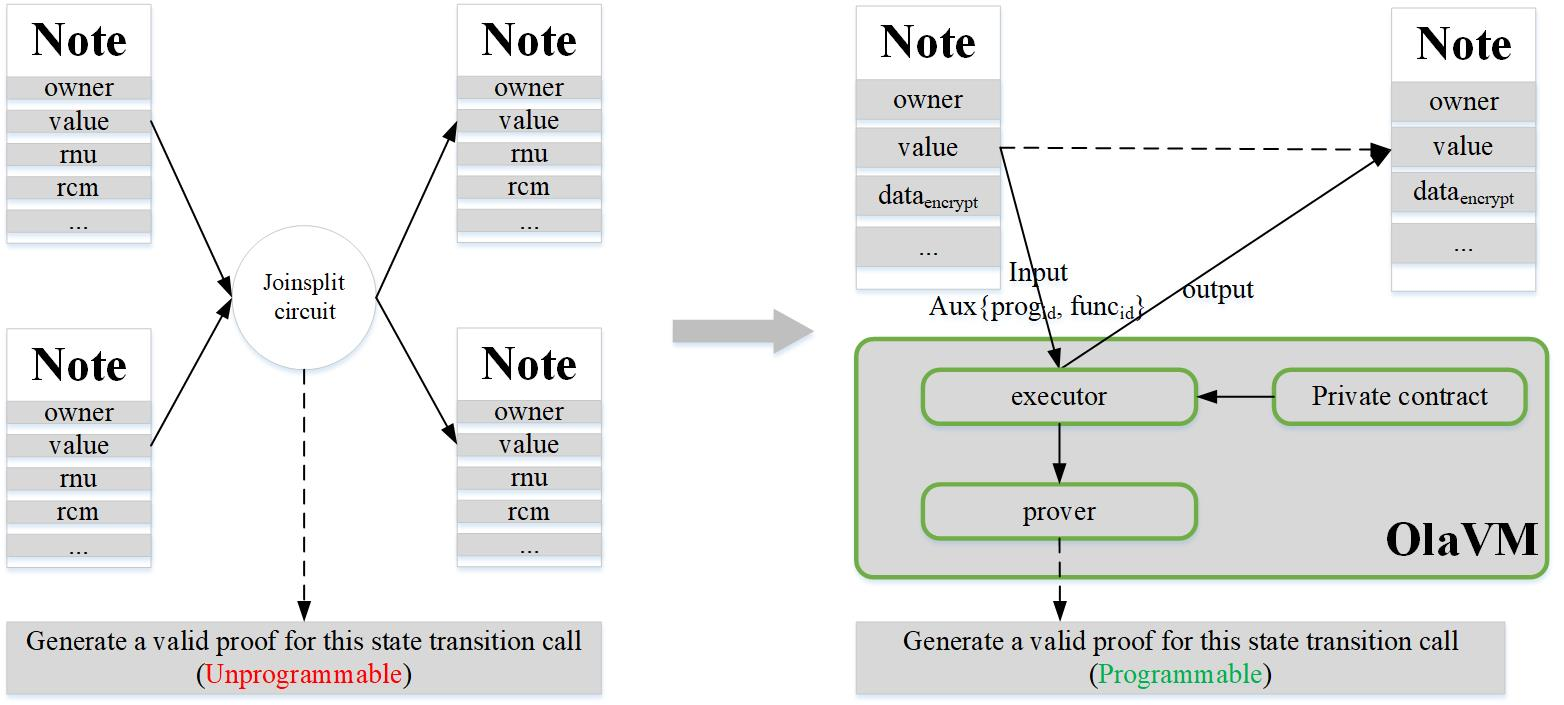
\includegraphics[width=0.6\textwidth]{Difference between Non Programmable Privacy and Programmable Privacy.jpg}
    \caption{Difference between Non Programmable Privacy and Programmable Privacy}
    \label{fig:Difference between Non Programmable Privacy and Programmable Privacy}
\end{figure}

The current projects focusing on programmable privacy are Aleo \cite{website:Aleo} and Aztec. Aleo is a 
privacy-first public blockchain, from Bitcoin \cite{website:BTC} to Ethereum to Zcash \cite{website:Zcash} to Aleo. It brings the public blockchain into a new era,
supporting programmable privacy. 
It has reached the testnet stage and supports developers to deploy privacy contracts on it; 
Aztec focuses on doing Layer2 programmable privacy for Ethereum, a project 
called Aztec3 \cite{website:Aztec3}, is still in development.

Before we clarify the different approaches to get programmability, we should give some explanations on Domain Specific Language (DSL) and General Purpose Language (GPL) \cite{website:DSL}.
DSL is defined as a computer programming language of limited expressiveness focused on a particular domain, limited expressiveness means it just supports a bare minimum of features 
needed to support its domain. You can't build an entire software system in a DSL; rather, you use a DSL for one particular aspect of a system. While GPL is defined as a general-purpose programming language

So there are often two ways to achieve programmability, one is to design a DSL, such as Circom \cite{website:Circom}, Pil \cite{website:Pil}, Noir \cite{website:Noir}, etc; the other is SCL, 
such as Cairo1.0 \cite{website:Cairo1.0}, Solidity \cite{website:Solidity}, Ola lang \cite{website:Ola-lang} and so on. As we have mentioned before, the main difference is that SCL supports more complex structures and has 
higher abstraction, it's more suitable for writing complex business logic and meanwhile, and DSL is more suitable for some simple computational expressions. 
Take Pil \cite{website:Pil} language as an example, you can directly use it to define a simple micro-op, such as ``A * B + C'', or ``A * B * C + D'' and other simple combinations. 
\tabref{table:Difference between DSL and SCL} briefly shows some of the differences between DSL and SCL.

\begin{table}[!ht]
    \centering
    \begin{tabular}{|c|c|c|c|c|c|}
        \hline
        \emph{Type} & \emph{Abstraction} & \emph{Process} & \emph{Difficulty} & \emph{Examples} & \emph{Notes} \\ 
        \hline
        DSL & low & program -> arith-ops -> ops gadgets & normal & \makecell{circom \\ noir \\ cairo} & \makecell{1. semantic analysis \\ 2. codeGen optimization} \\
        \hline
        \makecell{SCL \\ (ISA/VM)} & high & program -> bytecodes -> cpu circuit & hard & \makecell{solidity \\ cairo1.0 \\ ola lang} & \makecell{1. need a compiler \\2. re-use LLVM framework} \\
        \hline
    \end{tabular}
    \caption{Difference between DSL and SCL}
    \label{table:Difference between DSL and SCL}
\end{table}

If you want to prove a program written by DSL is executed correctly (this is what ZKDSL means), you may need to predefine some common operators, each of them corresponding to a circuit, called a gadget \cite{website:Gadget}. 
Developers can use these operators to implement desired functions, but it's difficult to handle the call and return logic between functions. Meanwhile, If you want to prove a program written by SCL is executed correctly (this is what ZKVM means), 
 you need to design corresponding constraints for each instruction, collectively referred to as CPU circuit; therefore, Any program will be compiled into 
 bytecodes composed of these instructions, and then constrained by the CPU circuit.

Ola achieved a customized SCL to get programmability even though it's harder to implement than DSL, because we could get benefits from it as follows:
 \begin{itemize}
 \item A higher abstraction and programmable language, allowing developers to write smart contracts with arbitrary logic;
 \item A full-featured zk-friendly VM can be designed to achieve higher system performance;
 \item LLVM-based compiler can be more easily compatible with other advanced programming languages.
\end{itemize}
